\chapter{Problema}

No contexto de simulações de fenômenos aeroacústicos usando Lattice Boltzmann, normalmente o campo de pressão ao longo do espaço é referente ao campo próximo e, por limitações de recursos computacionais, criar uma malha grande o suficiente para englobar o campo distante inviabiliza de forma integral a simulação. O presente problema a ser estudado e analisado diz respeito a um sólido quadrado que está sofrendo a influência de um escoamento de velocidade horizontal. O presente sistema é retratado de acordo com a figura \ref{fig1}.

\begin{figure}[h!]
    \centering
    \hspace{-1.cm}
    \label{fig1}
    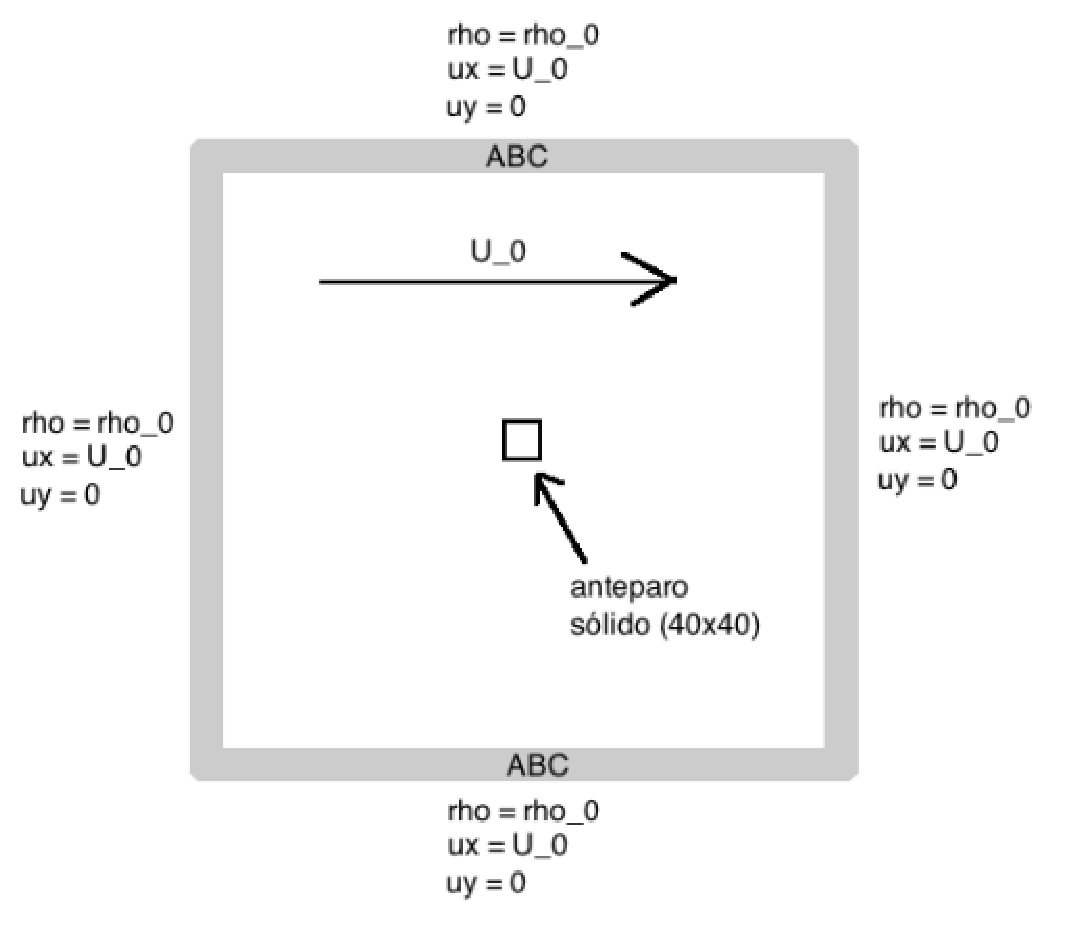
\includegraphics[width=0.5\textwidth]{../figuras/l5_1.eps}
    \caption{Esquemático do problema.}
\end{figure}

Diante do contexto exposto, propõe-se submeter esse sistema a um escomento de velocides Mach = 0.07 e 0.1. Além disso a superfície de FW-H será variada de 1 célula até 100 células de Lattice.

\chapter{Solução e Implementação}

Para mitigar esse problema há a proposta de \cite{lockard} que utiliza da superfície de Ffowcs Williams and Hawkings para extrapolar resultados para o campo distante usando a composição do espectro de frequências do campo acústico próximo.



\begin{figure}[h!]
    \centering
    \hspace{-1.cm}
    \label{fig1}
    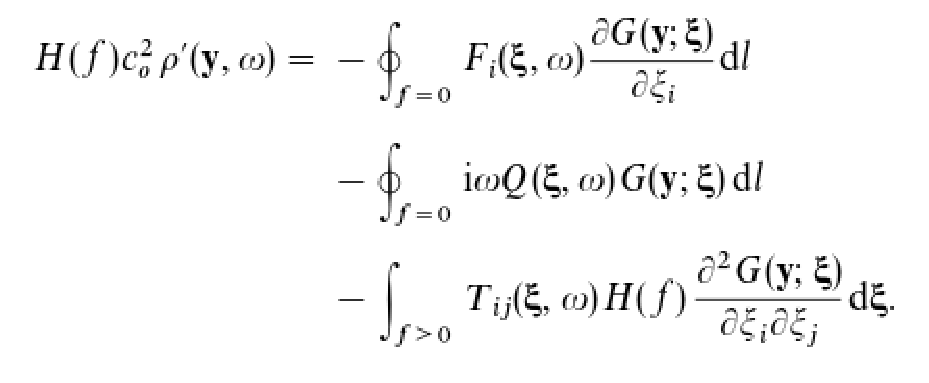
\includegraphics[width=0.5\textwidth]{../figuras/l5_2.eps}
    \caption{Equação da superfície de FW-H.}
\end{figure}

\chapter{Resultados}

